\documentclass{./../../Latex/teaching_slides}

\usepackage{venndiagram}
\usepackage{tikz}
\usepackage{caption}
\usepackage{subcaption}
\usepackage{pgfplots}
\pgfplotsset{compat=newest}
\usetikzlibrary{arrows.meta}

\begin{document}

\title{ECON 441 \\ \vspace{0.4em} \normalsize Introduction to Mathematical Economics}
\author{Div Bhagia}
\date{Midterm Review}

%%%%%%%%%%%%%%%%%%%%
\begin{frame}[noframenumbering, plain]
\maketitle
\end{frame}

\section{Numbers, Sets, and Functions}
%%%%%%%%%%%%%%%%%%%%%%%%%% Numbers, Sets, and Functions
%%%%%%%%%%%%%%%%%%%%
\begin{frame}{Sets}
\begin{witemize}
  \item $\mathbb{R}$ is the set of real numbers (rational and irrational)
  \item $x \in \mathbb{R}$ to denote $x$ belongs to the set of real numbers
  \item Consider the universe of all real numbers, set $A$ is given by:
  $$ A = \{x | x > 0\}$$
  \item What is the complement of $A$? \pause 
  $$ A^c = \{x | x \leq 0\}$$
  \end{witemize}
\end{frame}

%%%%%%%%%%%%%%%%%%%%
\begin{frame}{Set Relations and Operations}
Consider the following sets:
\begin{align*}
A &= \{x | x > 0\} \\
B &= \{x | x \text{ is a positive integer}\} \\
C &= \{x | 1<x<5\}
\end{align*}
\begin{itemize}
\item Is $A=B$? Is $B \subset A$? 
\item Are $C$ and $B$ disjoint sets?
\item What is $A \cap B$? What about $A \cup B$?
\item What is $B \cap C?$ 
\end{itemize}
\end{frame}

%%%%%%%%%%%%%%%%%%%%
\begin{frame}{Subsets}
\begin{itemize}
\item $\emptyset$: empty or null set \\~\\
\item  What are all possible subsets of $$S = \{a,b,c\}$$
\item[] $\emptyset, \{a\}, \{b\},\{c\}, \{a,b\}, \{b,c\}, \{a,c\}, \{a,b,c\}$  \\~\\
 Always $2^n$ subsets. Here $n=3$, so 8 subsets.
\end{itemize}
\end{frame}


%%%%%%%%%%%%%%%%%%%%
\begin{frame}{Set Operations: Venn Diagrams}
\vspace{1em}
\centering
\begin{venndiagram2sets}[tikzoptions={scale=0.75, thick}]
\end{venndiagram2sets}
\begin{venndiagram2sets}[tikzoptions={scale=0.75, thick}]
\end{venndiagram2sets} \\
\vspace{2.25em}
\begin{venndiagram2sets}[tikzoptions={scale=0.75, thick}]
\end{venndiagram2sets}
\end{frame}

%%%%%%%%%%%%%%%%%%%%
%\begin{frame}{Laws of Set Operations}
%\begin{itemize}
%\item Commutative law
%$$ A \cup B = B \cup A \quad \quad  A \cap B = B \cap A$$ \\~\\
%\item Distributive law
%$$ A \cup (B \cap C) = (A \cup B) \cap (A \cup C) $$
%$$ A \cap (B \cup C) = (A \cap B) \cup (A \cap C) $$
%\end{itemize}
%\end{frame}

%%%%%%%%%%%%%%%%%%%%
\begin{frame}{Cartesian Product}
$$ A = \{1,2\} \quad B = \{3,4\} $$ \\~\\
Cartesian Product: set of all possible ordered pairs
$$ A \times B = \{ (1,3), (1,4), (2,3), (2,4) \} $$
\end{frame}

%%%%%%%%%%%%%%%%%%%%
\begin{frame}{Cartesian Plane}
\vspace{-1em}
$$ \mathbb{R}^2 =  \{(x,y) | x \in \mathbb{R}, y \in \mathbb{R}\} $$
\centering
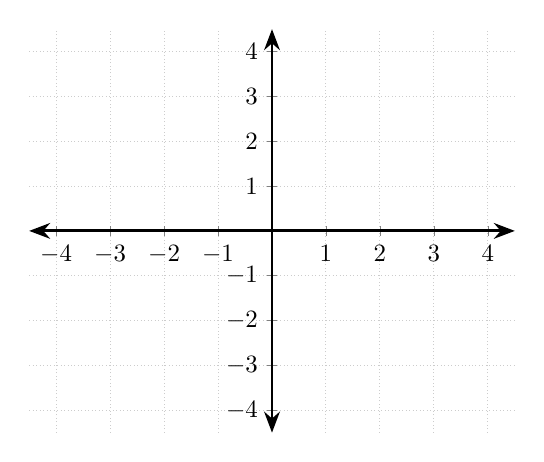
\begin{tikzpicture}[scale=0.9]
\begin{axis}[
  axis lines=middle,
  axis line style={Stealth-Stealth,very thick},
  xmin=-4.5,xmax=4.5,ymin=-4.5,ymax=4.5,
  xtick distance=1,
  ytick distance=1,
  %xlabel=$x$,
  %ylabel=$y$,
  %title={Wonderful plot},
  grid=major,
  grid style={thin,densely dotted,black!20}]
%\addplot [Latex-Latex,domain=-5:3,samples=2] {x*2/3} node[right]{$a$};
\end{axis}
\end{tikzpicture} \\~\\
\hspace{-3cm} Can have $ \mathbb{R}^3, \mathbb{R}^4,...,\mathbb{R}^n $
\end{frame}


%%%%%%%%%%%%%%%%%%%%
\begin{frame}{Relations}
Relation: subset of the Cartesian product \\~\\
Example. $\{(x,y) | y \leq x \} $

\centering
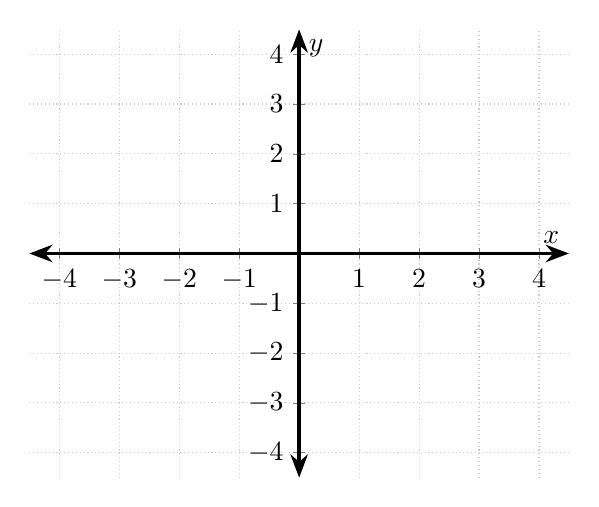
\begin{tikzpicture}
\begin{axis}[
  axis lines=middle,
  axis line style={Stealth-Stealth,very thick},
  xmin=-4.5,xmax=4.5,ymin=-4.5,ymax=4.5,
  xtick distance=1,
  ytick distance=1,
  xlabel=$x$,
  ylabel=$y$,
  %title={Wonderful plot},
  grid=major,
  grid style={thin,densely dotted,black!20}]
%\addplot [Latex-Latex,domain=-5:3,samples=2] {x*2/3} node[right]{$a$};
\end{axis}
\end{tikzpicture}
\end{frame}

%%%%%%%%%%%%%%%%%%%%
\begin{frame}{Functions}
 Function: a relation where for each $x$ there is a unique $y$  
$$ f: X \rightarrow Y, \quad y = f(x) $$ \\~\\
Examples. $y = x, y=x^2, y=2x+3 $ \\~\\

$X:$ domain, $Y:$ codomain, $f(X):$ range \\~\\

Most functions we will encounter, $f: \mathbb{R}^k \rightarrow \mathbb{R}$

\end{frame}

%%%%%%%%%%%%%%%%%%%%
\begin{frame}{Inverse of a function}
Function $y=f(x)$ has an inverse if it is a one-to-one mapping, i.e. each value of $y$ is associated with a unique value of $x$. \\~\\
Inverse function $$x=f^{-1}(y)$$ returns the value corresponding value of $x$ for each $y$. \\~\\
One-to-one mapping unique to strictly monotonic functions
\end{frame}


\pgfplotsset{%
    width=10cm,
    height=8cm
}


%%%%%%%%%%%%%%%%%%%%
\begin{frame}{$y=exp(x)$}
\centering
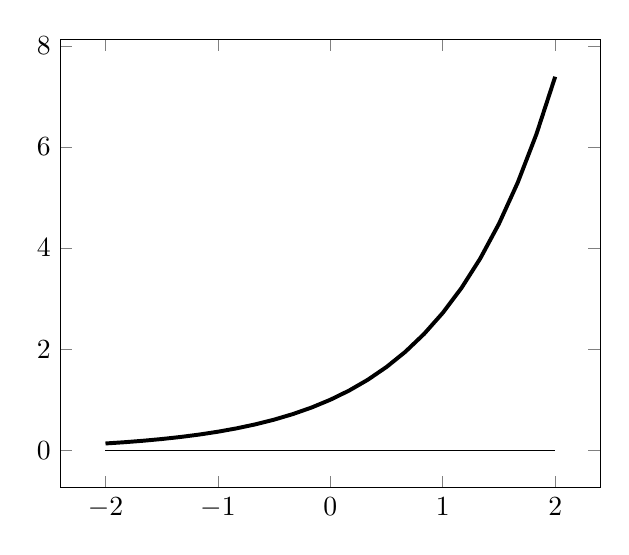
\begin{tikzpicture}
\begin{axis}[]
\addplot[color=black, line width=0.5mm, domain=-2:2] {exp(x)};
\addplot[domain=-2:2] {0};
\end{axis}
\end{tikzpicture} 
\end{frame}

%%%%%%%%%%%%%%%%%%%%
\begin{frame}{Logarithmic Function}
Since the exponential function is a monotonic function, its inverse exists. \\~\\
The inverse of the exponential function is called the log or logarithmic function. \\~\\
For the natural exponential function:
\[y=e^{t} \rightarrow \log _{e} y =ln(y) \]
\end{frame}

%%%%%%%%%%%%%%%%%%%%
\begin{frame}{$y=ln(x)$}
\centering
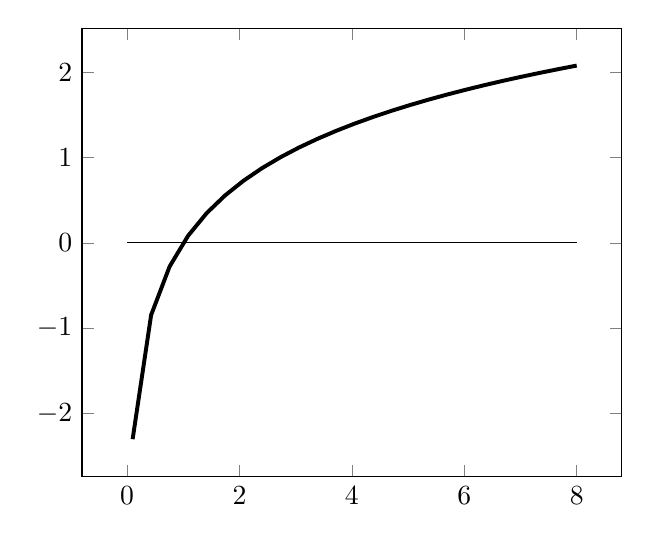
\begin{tikzpicture}
\begin{axis}[]
\addplot[color=black, line width=0.5mm, domain=0.1:8] {ln(x)};
\addplot[domain=0:8] {0};
\end{axis}
\end{tikzpicture} 
\end{frame}

%%%%%%%%%%%%%%%%%%%%
\begin{frame}{Rules for Logarithmic Functions}
\begin{itemize}
	\item[] $$\ln (u v)=\ln u+\ln v$$
	\item[] $$\ln (u / v)=\ln u-\ln v$$
	\item[] $$\ln u^{a}=a \ln u$$
\end{itemize}
\end{frame}


%%%%%%%%%%%%%%%%%%%%%%%%%%%% Add summation notation here as well 

%%%%%%%%%%%%%%%%%%%%%%%%%%%% Linear Algebra

\section{Linear Algebra}

%%%%%%%%%%%%%%%%%%%%
\begin{frame}{Matrices}
$$A = \begin{bmatrix}
a_{11} & a_{12}  & \hdots & a_{1n} \\
a_{21} & a_{22}  & \hdots & a_{2n} \\
\vdots & \vdots  & \vdots & \vdots \\
a_{m1} & a_{m2}  & \hdots & a_{mn} \\
\end{bmatrix}_{m \times n}$$

\vspace{1em}
Can write it more compactly
$$ A = [ a_{ij} ] \quad i=1,2,...,m; j=1,2,...,n$$ 

\textit{Square matrices}: $m=n$
\end{frame}

%%%%%%%%%%%%%%%%%%%%
\begin{frame}{Matrices}
Two matrices are \textit{equal} if all their elements are identical. \\~\\
Example.
$$A = \begin{bmatrix}
1 & 8  \\
4 &-1  \\
\end{bmatrix} \neq
 \begin{bmatrix}
1 & 8  \\
4 & 2  \\
\end{bmatrix}$$

\vspace{2em}
So $A=B$ if and only if $a_{ij} = b_{ij}$ for all $i, j$
\end{frame}

%%%%%%%%%%%%%%%%%%%%
\begin{frame}{Matrix Addition and Subtraction}
\begin{witemize}
\item How to add or take the difference between two matrices? 
\item[] \hspace{1em} $\rightarrow$ Element-by-element
\item[] \hspace{1em} $\rightarrow$  Matrices have to have same dimension \\~\\
\end{witemize}
Example.
$$A = \begin{bmatrix}
2 & 3 \\
4 & -6 
 \end{bmatrix} \quad \quad
B = \begin{bmatrix}
1 & 8 \\
-2 & 3
\end{bmatrix}$$
\begin{witemize}
\item What is $A+B$ and $A-B$?
\end{witemize}
\end{frame}

%%%%%%%%%%%%%%%%%%%%
\begin{frame}{Scalar Multiplication}
How to multiply a scalar to a matrix? 
$$ \lambda \begin{bmatrix} a_{11} & a_{12} & a_{13} \\ 
a_{21} & a_{22} & a_{23} \\  \end{bmatrix} = \begin{bmatrix} \lambda a_{11} & \lambda a_{12} & \lambda a_{13} \\ 
\lambda a_{21} & \lambda a_{22} & \lambda a_{23} \\  \end{bmatrix} $$
Example.
$$A = \begin{bmatrix}
2 & 3 \\
4 & -6 
\end{bmatrix}  \quad \quad
B = \begin{bmatrix}
1 & 8 \\
-2 & 3
\end{bmatrix}$$
What is $2B$ and $A-2B$?
\end{frame}


%%%%%%%%%%%%%%%%%%%%
\begin{frame}{Matrix Multiplication}
Only possible to multiply two matrices, $A_{m \times n}$ and $B_{p \times q}$ to get $AB$ if $ n = p $ i.e.
$$\text{number of columns in } A = \text{ number of rows in } B $$ 
\\~\\

Example.
$A = \begin{bmatrix}
2 & 3  \\
4 & -6 
\end{bmatrix}_{2 \times 2}$ 
$B = \begin{bmatrix}
1 & 8 & 1\\
-2 & 3 & 1
\end{bmatrix}_{2 \times 3}$ \\~\\

\vspace{1em}
Can do $AB$, but cannot do $BA$. Dimension of $AB$ is $2 \times 3$.
\end{frame}




%%%%%%%%%%%%%%%%%%%%
\begin{frame}{Matrix Multiplication}
So how to actually multiply these matrices? 
$$ C = AB$$
$$ c_{ij} = a_{i1} b_{1j} + a_{i2} b_{2j} + ... + a_{in} b_{nj} = \sum_{k=1}^n a_{ik} b_{kj}   $$

\vspace{1em}
Element $c_{ij}$ obtained by multiplying term-by-term the entries of the $i$th row of $A$ and $j$th column of $B$. 
\end{frame}

%%%%%%%%%%%%%%%%%%%%
\begin{frame}{Matrix Multiplication}
$$A = \begin{bmatrix}
2 & 3  \\
4 & -6 
\end{bmatrix}_{2 \times 2} \quad B = \begin{bmatrix}
1 & 8 & 1\\
-2 & 3 & 1
\end{bmatrix}_{2 \times 3}$$
\end{frame}


%%%%%%%%%%%%%%%%%%%%
\begin{frame}{Vectors}
\begin{witemize}
\item Matrices with only one column: column vectors 
$$ x =  \begin{bmatrix}
x_1\\
x_2 \\
\vdots \\
x_n
\end{bmatrix} $$
\item Matrices with only one row: row vectors
$$ x' =  \begin{bmatrix}
x_1 &
x_2 & \hdots &
x_n
\end{bmatrix} $$
\end{witemize}
\end{frame}

%%%%%%%%%%%%%%%%%%%%%
%\begin{frame}{Inner Product}
%Inner product of two vectors each with $n$ elements:
%$$ u \cdot v = u_1 v_1 + u_2 v_2 +...+ u_n v_n = \sum_{i=1}^n u_i v_i $$ 
%Example. $$u = \begin{bmatrix} 1 \\ 5 \\ 2 \end{bmatrix} \quad \quad v = \begin{bmatrix} 2 \\ 1 \\ 3 \end{bmatrix}$$
%\end{frame}

%%%%%%%%%%%%%%%%%%%%
\begin{frame}{Linear Dependence}
A set of vectors is said to be \textit{linearly dependent} if and only if any one of them can be expressed as a linear combination of the remaining vectors. \\~\\
Example.$$ v_1 =  \begin{bmatrix}
1\\
2 \\
\end{bmatrix} \quad \quad v_2 = \begin{bmatrix}
2\\
4 \\
\end{bmatrix}$$
\end{frame}


%%%%%%%%%%%%%%%%%%%%
\begin{frame}{Identity Matrices}
Square matrix with $1$s in its \textit{principal diagonal} and $0$s elsewhere \\~\\
A $2 \times 2$ identity matrix:
$$ I_2 = \begin{bmatrix}
1 & 0\\
0 & 1 \\
\end{bmatrix}$$
A $3 \times 3$ identity matrix:
$$ I_3 = \begin{bmatrix}
1 & 0 & 0 \\
0 & 1 & 0\\
0 & 0 & 1
\end{bmatrix}$$

\end{frame}

%%%%%%%%%%%%%%%%%%%%
\begin{frame}{Identity Matrices}
Acts like 1, 
$$ AI = IA = A $$

\vspace{2em}

Example. 
$$A = \begin{bmatrix}
2 & 3 & 1 \\
4 & -6 & 2
\end{bmatrix}$$
\end{frame}


%%%%%%%%%%%%%%%%%%%%
\begin{frame}{Transpose of a Matrix}
Transpose of A: interchange rows and columns ($A'$) \\~\\
$$A = \begin{bmatrix}
2 & 3 & 1 \\
4 & -6 & 2
\end{bmatrix}$$
\end{frame}

%%%%%%%%%%%%%%%%%%%%
%\begin{frame}{Properties of Transposes}
%$$
%\begin{array}{l}
%\left(A^{\prime}\right)^{\prime}=A \\~\\
%(A+B)^{\prime}=A^{\prime}+B^{\prime} \\~\\
%(A B)^{\prime}=B^{\prime} A^{\prime} \\~\\
%\end{array}
%$$
%Example:
%\( A=\left[\begin{array}{ll}4 & 1 \\ 9 & 0\end{array}\right] \quad B=\left[\begin{array}{ll}2 & 0 \\ 7 & 1\end{array}\right] \)
%\end{frame}

%%%%%%%%%%%%%%%%%%%%
\begin{frame}{Inverse of a Matrix}
For a \textbf{square} matrix $A$, it's inverse $A^{-1}$ is defined as:
$$
A A^{-1}=A^{-1} A=I
$$

\vspace{2em}
 Squareness is a \textit{necessary} condition not a \textit{sufficient} condition \\~\\
 If a matrix's inverse exists, it's called a \textbf{nonsingular} matrix
\end{frame}

%%%%%%%%%%%%%%%%%%%%%
%\begin{frame}{Properties of Inverses}
%$$ \left(A^{-1}\right)^{-1}=A $$ \\~\\
%$$ (A B)^{-1}=B^{-1} A^{-1} $$ \\~\\
%$$ \left(A^{\prime}\right)^{-1}=\left(A^{-1}\right)^{\prime} $$
%\end{frame}

%%%%%%%%%%%%%%%%%%%%
\begin{frame}{Conditions for Nonsingularity}
Squareness is \textit{necessary} but not  \textit{sufficient} \\~\\
Sufficient condition for nonsingularity: \\~\\
\hspace{1em} \textit{Rows or columns are linearly independent} \\~\\
Example. $$
A=\left[\begin{array}{ll}
1 & 2 \\
2 & 4
\end{array}\right]
\quad
B=\left[\begin{array}{ll}
1 & 2 \\
3 & 4
\end{array}\right]
$$
\pause $A$ is singular, $B$ is nonsingular.
\end{frame}


%%%%%%%%%%%%%%%%%%%%
\begin{frame}{Rank of a Matrix}
Rank of a matrix $=$ maximum number of linearly independent rows \\~\\
$$A=\left[\begin{array}{ll}
1 & 2 \\
2 & 4
\end{array}\right]
\quad
B=\left[\begin{array}{ll}
1 & 2 \\
3 & 4
\end{array}\right]
$$
\vspace{1em}

Rank of $A$? Rank of $B$? \\~\\

Full rank = all rows linearly independent =nonsingular matrix
\end{frame}



 %%%%%%%%%%%%%%%%%%%%
\begin{frame}{Determinant}
 Determinant $|A|$ is a unique scalar associated with a \textit{square} matrix $A$. \\~\\
 $|A|=0$ for a singular matrix. \\~\\
 Determinant of a $2 \times 2$ Matrix:
 $$ A=\left[\begin{array}{ll}a_{11} & a_{12} \\ a_{21} & a_{22}\end{array}\right] $$
 Can be calculated as:
 $$ |A|=a_{11} a_{22}-a_{12} a_{21} $$  
 \end{frame}
 
   %%%%%%%%%%%%%%%%%%%%
%\begin{frame}{Determinant of a $3 \times 3$ Matrix}
%$$
%\begin{aligned}
%|A| &=\left|\begin{array}{lll}
%a_{11} & a_{12} & a_{13} \\
%a_{21} & a_{22} & a_{23} \\
%a_{31} & a_{32} & a_{33}
%\end{array}\right| \\~\\
%&=a_{11}\left|\begin{array}{ll}
%a_{22} & a_{23} \\
%a_{32} & a_{33}
%\end{array}\right|-a_{12}\left|\begin{array}{ll}
%a_{21} & a_{23} \\
%a_{31} & a_{33}
%\end{array}\right| 
%+a_{13}\left|\begin{array}{ll}
%a_{21} & a_{22} \\
%a_{31} & a_{32}
%\end{array}\right|
%\end{aligned}
%$$
% \end{frame}
 
    %%%%%%%%%%%%%%%%%%%%
\begin{frame}{Determinant of a $n \times n$ Matrix}
A \textit{minor} of the element $a_{ij}$, denoted by $|M_{ij}|$ is obtained by deleting the $i$th row and $j$th column. \\~\\
Cofactor $C_{ij}$ is defined as:
$$ |C_{ij}| = (-1)^{i+j} |M_{ij}| $$
 Then, 
 $$|A| = \sum_{i=1}^n a_{ij} |C_{ij}| = \sum_{j=1}^n a_{ij} |C_{ij}| $$
 \end{frame}
 
%%%%%%%%%%%%%%%%%%%%
\begin{frame}{Find the Determinant}
\[
A=\left[\begin{array}{ccc}
1 & 5 & 1 \\
0 & 3 & 9 \\
-1 & 0 & 0
\end{array}\right]
\]
 \end{frame}


 
% %%%%%%%%%%%%%%%%%%%%
%\begin{frame}{Properties of Determinants}
%\vspace{-0.5em}
%\begin{witemize}
%\item[1.] $ |A| = |A'|$ 
%\item[2.] Interchanging rows or columns will alter the sign but not the value
%\item[3.] Multiplication of any one row (or one column) by a scalar $k$ will change the value of the determinant $k$-fold
%\item[4.] The addition (subtraction) of a multiple of any row (or column) to (from) another row (or column) will leave the determinant unaltered
%\item[5.] If one row (or column) is a multiple of another row (or column), the value of the determinant will be zero. 
%\end{witemize}
% \end{frame}
% 
 %%%%%%%%%%%%%%%%%%%%
\begin{frame}{Matrix Inversion}
 \textit{Adjoint} of a nonsingular $n \times n$ matrix \\~\\
 $$adj A = C' = \left[\begin{array}{llll}
|C_{11}| & |C_{21}| & \hdots & |C_{n1}| \\
|C_{12}| & |C_{22}| & \hdots &  |C_{n2}| \\
\vdots &\vdots & \hdots &  \vdots \\
|C_{1n}| & |C_{2n}| & \hdots & |C_{nn}| \\
\end{array}\right]$$
\vspace{1em}
$$ A^{-1} = \frac{1}{|A|} Adj A$$
 \end{frame}

%%%%%%%%%%%%%%%%%%%%
\begin{frame}{Find the Inverse}
$$
A=\left[\begin{array}{ccc}
3 & 2 \\
1 & 0 \\
\end{array}\right]
$$
 \end{frame}

%%%%%%%%%%%%%%%%%%%%
\begin{frame}{A Simple Economic Model}
Two equations in two unknowns:
\begin{align*}
q + 2p &= 100 \\ q-3p &= 20
\end{align*}
Can write this as:
$$ Ax = b $$
where
$$A = \begin{bmatrix}
1 & 2 \\
1 & -3 
\end{bmatrix} \quad 
x = \begin{bmatrix}
q \\
p 
\end{bmatrix} \quad 
b = \begin{bmatrix}
100 \\
20 
\end{bmatrix}$$
\end{frame}

%%%%%%%%%%%%%%%%%%%%
\begin{frame}{Solution of Linear-Equation System}
$$ Ax = b $$

\vspace{0.5em}
Pre-multiply both sides by $A^{-1}$, 
$$ A^{-1} Ax = A^{-1} b \quad \implies x = A^{-1} b $$

What happens if $A$ is singular? Infinite solutions.
\end{frame}

%%%%%%%%%%%%%%%%%%%%%
%\begin{frame}{Homogeneous equation system}
%A homogeneous equation system is given by 
%$$ Ax = 0$$
%If $A$ is nonsingular, $x^* = A^{-1} 0 = 0$. \\~\\
% If $A$ is singular there can be infinite number of solutions (this is true for any system of equations).
%\end{frame}

%%%%%%%%%%%%%%%%%%%%%
%\begin{frame}{An Application of Matrix Algebra}
%Linear regression model:
%  $$ Y_i = \beta_0 + \beta_1 X_{1,i} + \beta_2 X_{2,i} + \hdots + \beta_{k} X_{k,i}  + \varepsilon_i $$ 
%Denote, \small 
%$$ Y  = \begin{bmatrix} Y_1 \\ Y_2 \\ \vdots \\ Y_n  \end{bmatrix}_{n \times 1}    
%  \beta  = \begin{bmatrix} \beta_0 \\ \beta_1 \\ \vdots \\ \beta_{k}  \end{bmatrix}_{(k+1) \times 1}  
%  \boldsymbol{X} = \begin{bmatrix} 
%  	1 & X_{1,1} & \hdots & X_{k,1} \\ 
%  	1 & X_{1,2} & \hdots  & X_{k,2} \\
%   \vdots & \vdots & \hdots &  \vdots \\ 
%   1 & X_{1,n}  & \hdots & X_{k,n} \end{bmatrix}_{n \times (k+1)} 
%   \varepsilon = \begin{bmatrix} \varepsilon_1 \\ \varepsilon_2 \\ \vdots \\ \varepsilon_n  \end{bmatrix}_{n \times 1}$$
%   \normalsize
%   Can write the model as: $$ Y = X\beta + \varepsilon $$
%\end{frame}
%
%%%%%%%%%%%%%%%%%%%%%
%\begin{frame}{An Application of Matrix Algebra}
%Linear regression model:
%$$ Y = X\beta + \varepsilon $$
%Ordinary least squares estimator: $\beta$ that minimizes
%$$ \varepsilon'\varepsilon = (Y-X\beta)'(Y-X\beta) $$
%Few lines of calculus: 
%$$ \hat{\beta} = (X'X)^{-1}(X'Y) $$
%\end{frame}
%
%%%%%%%%%%%%%%%%%%%%%
%\begin{frame}{Another Application of Matrix Algebra}
%In network theory, represent network as a matrix. \\~\\
%For example, consider 3 banks. Below is a matrix representing connectedness between banks:
%$$ M  = \begin{bmatrix} 
%0 & 1 & 0 \\ 
%0 & 0 & 1 \\
%0 & 0 & 0 
%\end{bmatrix} $$
%$M_{ij}$ is 1 if $i$ has lent to $j$. So bank 1 has lent to bank 2 and bank 2 has lent to bank 3. What if bank 3 fails? Look at $M^2$.
%\end{frame}

%%%%%%%%%%%%%%%%%%%%%%%%%%%% Calculus
\section{Calculus}

%%%%%%%%%%%%%%%%%%%%
\begin{frame}{Differentiability and Continuity}
$f'(x_0)$ exists if the following limit exists: 
$$  f'(x_0)= \lim_{ x \rightarrow x_0} \frac{f(x)-f(x_{0})}{x-x_0}  $$


\vspace{1em}
A function $y=f(x)$ is continuous at $x_0$ if $$\lim _{x \rightarrow x_0} f(x) = f(x_0)$$

Continuity is a necessary condition for differentiability, but it is not sufficient.
\end{frame}

%%%%%%%%%%%%%%%%%%%%
\begin{frame}{So how to differentiate functions?}
Rules of differentiation, easier than taking the limit each time \\~\\
\textit{Constant function rule:}\\
For function \(f(x)=k \), $ f'(x)=0 $.\\~\\
\textit{Power function rule:}\\
For function \( f(x)=x^{n} \), \( f^{\prime}(x)=n x^{n-1} \).\\~\\
\textit{Generalized power function rule:}\\
For function \( f(x)=c x^{n} \), \( f^{\prime}(x)=c n x^{n-1} \).
\end{frame}

%%%%%%%%%%%%%%%%%%%%
\begin{frame}{Derivatives of Exponential and Logarithmic Functions}
Derivative of the exponential function:
 $$y=e^x \quad \rightarrow \quad \frac{dy}{dx} = e^x$$
 
Derivative of the log function:
 $$y=\ln x \quad \rightarrow \quad \frac{dy}{dx} = \frac{1}{x}$$
\end{frame}

%%%%%%%%%%%%%%%%%%%%
\begin{frame}{Rules of Differentiation}
\underline{Two or more functions of one variable} \\~\\ 
\textit{Sum-Difference Rule}
$$ \frac{d}{d x}[f(x) \pm g(x)]=f^{\prime}(x) \pm g^{\prime}(x) $$\\~\\

\textit{Product Rule} \\
$$
\frac{d}{d x}[f(x) g(x)]=f(x) g^{\prime}(x)+f^{\prime}(x) g(x)
$$
\end{frame}

%%%%%%%%%%%%%%%%%%%%
\begin{frame}{Rules of Differentiation}
\underline{Two or more functions of one variable} \\~\\ 
\textit{Quotient Rule}\\
$$ \frac{d}{d x} \frac{f(x)}{g(x)}=\frac{f^{\prime}(x) g(x)-f(x) g^{\prime}(x)}{g(x)^2} $$\\~\\
\textit{Inverse Function Rule}
$$
\frac{d x}{d y}=\frac{1}{d y / d x}
$$

\end{frame}


%%%%%%%%%%%%%%%%%%%%
\begin{frame}{Rules of Differentiation}
\underline{Functions of Different Variables} \\~\\
\textit{Chain Rule} \\
\vspace{0.5em}
For \( z=f(y), \quad y=g(x) \)
$$ \frac{d z}{d x}=\frac{d z}{d y} \cdot \frac{d y}{d x}=f^{\prime}(y) g^{\prime}(x) $$ \\~\\
\end{frame}


%%%%%%%%%%%%%%%%%%%%
\begin{frame}{Example}
Total cost: $C=C(Q)$ \\~\\
Marginal cost: $MC = C'(Q)$ \\~\\
Average cost:
$$ AC = \frac{C(Q)}{Q} $$ \\~\\
When is $ \frac{d AC}{d Q} $ positive?
\end{frame}


%%%%%%%%%%%%%%%%%%%%
\begin{frame}{Example}
Revenue: $R=f(Q), \quad f'(Q)>0$ \\~\\
Output: $Q = g(L), \quad g'(L)>0$ \\~\\
Change in revenue due to labor adjustment:
$$ \frac{d R}{d L} = \frac{d R}{d Q} \cdot \frac{d Q}{d L} = f'(Q) g'(L) $$ \\~\\
\end{frame}

%%%%%%%%%%%%%%%%%%%%
\begin{frame}{Elasticity}
Elasticity is defined as:
\[ \varepsilon = \frac{\text{Percentage change in y}}{\text{Percentage change in x}} = \frac{dy/y}{dx/x} \] \\

We can calculate this as:
\[ \varepsilon = \frac{dy}{dx} \cdot \frac{x}{y} \]
\end{frame}

%%%%%%%%%%%%%%%%%%%%
\begin{frame}{Elasticity}
Elasticity: 
\[ \varepsilon = \frac{dy}{dx} \cdot \frac{x}{y} \]
\vspace{1cm}
\begin{itemize}
	\item $|\varepsilon|>1$, elastic
	\item $|\varepsilon|=1$, unit elasticity
	\item $|\varepsilon|<1$, inelastic
\end{itemize}
\end{frame}

%%%%%%%%%%%%%%%%%%%%
\begin{frame}{Example}
$$ C = a + bY $$
\end{frame}


%%%%%%%%%%%%%%%%%%%%
\begin{frame}{Partial Differentiation}

For a function of several variables:
$$
y=f\left(x_{1}, x_{2}, \cdots, x_{n}\right)
$$

If $x_1$ changes by $\Delta x_1$ but all other variables remain constant: 
$$
\frac{\Delta y}{\Delta x_{1}}=\frac{f\left(x_{1}+\Delta x_1, x_{2}, \cdots, x_{n}\right)-f\left(x_{1}, x_{2}, \cdots, x_{n}\right)}{\Delta x_{1}}
$$
Partial derivative of $y$ with respect to $x_i$:
$$
\frac{\partial y}{\partial x_{i}}= f_i = \lim _{\Delta x_{i} \rightarrow 0} \frac{\Delta y}{\Delta x_{i}}
$$
\end{frame}

%%%%%%%%%%%%%%%%%%%%
\begin{frame}{Production Function}
$$ Q = A K^{\alpha} L^{1-\alpha} $$ \\~\\

Marginal product of capital (MPK):
	$$\frac{\partial Q}{ \partial K} = Q_K =  \hspace{5cm} $$

Marginal product of labor (MPL):
	$$\frac{\partial Q}{ \partial L} = Q_L =  \hspace{5cm} $$
\end{frame}

%%%%%%%%%%%%%%%%%%%%
\begin{frame}{Total Derivative}
For a function of $n$ variables \[y=f\left(x_{1}, x_{2}, \cdots, x_{n}\right)\]

\[
\frac{d f}{d t}= f_1 \cdot \frac{d x_{1}}{d t} +f_2\cdot \frac{d x_{2}}{d t}+\cdots+f_n \cdot\frac{d x_{n}}{d t} \]
\end{frame}

%%%%%%%%%%%%%%%%%%%%
\begin{frame}{Total Derivative}
Given the function 
\[ y = f(x_1, x_2) \]

We are interested in how $y$ changes with respect to $x_1$, but $x_2$ also depends of $x_1$
\[ x_2 = g(x_1) \]

Total derivative with respect to $x_1$:
\[ \frac{dy}{dx_1} =  f_1+f_2 \cdot g'(x_1)   \]

\end{frame}

%%%%%%%%%%%%%%%%%%%%
\begin{frame}{Example}
Let a production function be
$$
Q(t) = A(t) K(t)^{\alpha} L(t)^{1-\alpha} 
$$
where 
$$
K(t) = K_0 + at  \quad \quad L(t) = L_0 + bt
$$
\end{frame}


%%%%%%%%%%%%%%%%%%%%
\begin{frame}{Gradient}
For the function:
$$ y = f(x_1, x_2,...,x_n) $$ 
\vspace{0.5em}

The gradient is given by
$$ \nabla f = \begin{bmatrix}
	f_1 \\
	f_2 \\
	\vdots \\
	f_n
\end{bmatrix} $$
\end{frame}

%%%%%%%%%%%%%%
\begin{frame}{Derivatives of Implicit Functions}

Total differentiating $F$, we have $d F=0$, or
$$
F_{y} d y+F_{1} d x_{1}+\cdots+F_{n} d x_{n}=0 
$$

\vspace{1em}
Suppose that only $y$ and $x_{1}$ are allowed to vary:
$$
\frac{\partial y}{\partial x_{1}}=-\frac{F_{1}}{F_{y}} .
$$

\vspace{1em}
In the simple case where the given equation is $F(y, x)=0$, the rule gives
$$
\frac{d y}{d x}=-\frac{F_{x}}{F_{y}} .
$$
\end{frame}

%%%%%%%%%%%%%%%%%%%%
\begin{frame}{Example}
$$ Y = \beta_0 + \beta_1 \ln X + u $$ \\~\\

What is the interpretation of $\beta_1$?
\end{frame}


%%%%%%%%%%%%%%%%%%%%%
%\begin{frame}{Integration}
%\begin{witemize}
%  \item Integration is the reverse of differentiation 
%  \item If $f(x)$ is the derivative of $F(x)$, we can \textit{integrate} $f(x)$ to find $F(x)$
%  $$ \frac{d}{d x} F(x)=f(x) \Rightarrow \int f(x) d x=F(x)+c $$
%  \item Rules of integration follow from rules of differentiation
%\end{witemize}
%\end{frame}
%
%%%%%%%%%%%%%%%%%%%%%
%\begin{frame}{Rules of Integration}
%\underline{Power Rule}
%$$\int x^n d x=\frac{1}{n+1} \cdot x^{n +1} + c \quad(n \neq-1)$$
%
%\textit{Examples}: $$ \int x^3 d x , \quad \quad \int x d x, \quad  \quad \int 1 d x $$
%\end{frame}
%
%%%%%%%%%%%%%%%%%%%%%
%\begin{frame}{Rules of Integration}
%\underline{Exponential Rule}
%$$
%\int e^x d x=e^x+c
%$$
%
%\underline{Log Rule}
%$$
%\int \frac{1}{x} d x=\ln x+c \quad(x>0)
%$$
%\end{frame}
%
%%%%%%%%%%%%%%%%%%%%%
%\begin{frame}{Rules of Integration}
%\underline{Integral of a sum}
%$$
%\int[f(x)+g(x)] d x=\int f(x) d x+\int g(x) d x$$
%
%\underline{Integral of a multiple}
%$$\int k f(x) d x=k \int f(x) d x$$
%
%\textit{Example}: $$ \int (x^2 + 3x + 1) dx \hspace{7cm} $$
%\end{frame}
%
%%%%%%%%%%%%%%%%%%%%%
%\begin{frame}{Definite Integrals}
%Definite integral:
%$$ \left.\int_a^b f(x) d x=F(x)\right]_{a}^b=F(b)-F(a) $$
%\textit{Example}:  $$ \int_1^3 2 x^2 = \hspace{7cm}$$
%\end{frame}
%
%%%%%%%%%%%%%%%%%%%%%
%\begin{frame}{Area under the curve} 
%\vspace{0.5em}
%\begin{columns}[c]
%\begin{column}{0.6\textwidth}
%  	\begin{tikzpicture}[scale=0.9]
%  \begin{axis}[
%      axis lines = middle,
%      xlabel = \(x\), 
%      xlabel style={at={(axis description cs:1,0)}, anchor=west},
%      ylabel = {\(f(x)\)}, 
%      ylabel style={at={(axis description cs:0,0.95)}, anchor=east},
%      ymin=0,
%      xmin=0,
%      xmax=6,
%      ymax=30,
%      xtick={0.01,1.1,2.2,3.3, 4.4, 5.5},
%      xticklabels = {$x_0$, $x_1$, $x_2$, $x_3$, $x_4$, $x_5$},
%      ytick=\empty,
%      samples=100
%    ]
%    \addplot[ybar, ybar interval, fill=grey!30, domain=0:5.5, samples=6]{25+ x-x^2}\closedcycle;
%    \addplot[domain=0:6, black, very thick]{25+ x-x^2};
%  \end{axis}
%  \draw[decorate,decoration={brace,amplitude=4pt,mirror}, thick] (3.15,-0.65) -- (4.8,-0.65);
%  \node at (4,-1.25) {$\Delta x_3 $};
%    \node at (4,5.25) {$f(x_3) $};
%\end{tikzpicture}
%\end{column}	
%\begin{column}{0.4\textwidth}
% $ Area \approx \sum_{i=1}^n f(x_i) \Delta x_i $
%\end{column}	
%\end{columns}
%\end{frame}
%
%%%%%%%%%%%%%%%%%%%%%
%\begin{frame}{Area under the curve} 
%\vspace{1em}
%\begin{columns}[c]
%\begin{column}{0.5\textwidth}
%  	\begin{tikzpicture}[scale=0.9]
%  \begin{axis}[
%      axis lines = middle,
%      xlabel = \(x\), 
%      xlabel style={at={(axis description cs:1,0)}, anchor=west},
%      ylabel = {\(f(x)\)}, 
%      ylabel style={at={(axis description cs:0,0.95)}, anchor=east},
%      ymin=0,
%      xmin=0,
%      xmax=6,
%      ymax=30,
%      xtick=\empty,
%      ytick=\empty,
%      samples=100
%    ]
%    \addplot[ybar, ybar interval, fill=grey!30, domain=0:5.5, samples=20]{25+ x-x^2}\closedcycle;
%    \addplot[domain=0:6, black,  very thick]{25+ x-x^2};
%    
%  \end{axis}
%\end{tikzpicture}
%\end{column}	
%\begin{column}{0.5\textwidth}
%\begin{align*}
%	Area &= \lim_{n \rightarrow \infty} \sum_{i=1}^n f(x_i) \Delta x_i \\
%	& = \int_{x_1}^{x_n} f(x) dx
%\end{align*}  
%\end{column}	
%\end{columns}
%\end{frame}


%%%%%%%%%%%%%%%%%%%%
\begin{frame}{Few last words}
\begin{witemize}
\item Sample exam, midterm exams from previous semesters, and help sheet on course website
\item Note: We skipped integration so ignore slides after slide 15 in Lecture 7 and homework problems from chapter 14.
%  \item Additional office hours this week: Thursday, 4-6 pm. Or by appointment.
  \item Good luck for the exam!
\end{witemize}
\end{frame}

\end{document}